%%
%% Packages.tex
%% Login : <hoang-trong@hoang-trong-laptop>
%% Started on  Fri Jun 12 19:41:23 2009 Hoang-Trong Minh Tuan
%% $Id$
%% 
%% Copyright (C) 2009 Hoang-Trong Minh Tuan
%% This program is free software; you can redistribute it and/or modify
%% it under the terms of the GNU General Public License as published by
%% the Free Software Foundation; either version 2 of the License, or
%% (at your option) any later version.
%% 
%% This program is distributed in the hope that it will be useful,
%% but WITHOUT ANY WARRANTY; without even the implied warranty of
%% MERCHANTABILITY or FITNESS FOR A PARTICULAR PURPOSE.  See the
%% GNU General Public License for more details.
%% 
%% You should have received a copy of the GNU General Public License
%% along with this program; if not, write to the Free Software
%% Foundation, Inc., 59 Temple Place, Suite 330, Boston, MA 02111-1307 USA
%%

\chapter{Packages}
\label{chap:packages}


\section{Dealing with a package}
\label{sec:dealing-with-package}

\subsection{Install a package}
\label{sec:install-package-1}


To install a package\footnote{\url{http://support.stat.ucla.edu/view.php?supportid=30 
}}.

\begin{lstlisting}
> install.packages("package_name")
\end{lstlisting}

Example: the {\it aplpack} package 
\begin{lstlisting}
> install.packages("aplpack")
\end{lstlisting}

\subsection{Load/Unload an installed package}
\label{sec:load-an-inst}

In R, there are many user defined packages. The system has some
automatically loadded/attached packages: base, stats, datasets...
\begin{table}
\begin{center}
  \begin{tabular}{cl}
    graphics & all functions to produce graphics \\
    grDevices & all functions to handle different devices for graphics
    \\
    datasets & objects from different sample data sets \\
    utils  & all standard R utility functions \\
    stats & all standard R functions for statistical data analysis \\
  \end{tabular}
\end{center}
\caption{Standard packages}
\end{table}


\textbullet List all loaded packages with {\bf search()}
\begin{lstlisting}
>> search() 
[1] ".GlobalEnv"        "package:stats"     "package:graphics" 
[4] "package:grDevices" "package:utils"     "package:datasets" 
[7] "package:methods"   "Autoloads"         "package:base" 
\end{lstlisting}
The first location, the package with index = 1, is always.GlobalEnv.

\textbullet List all loaded packages with {\bf sessionInfo()}
\begin{lstlisting}
>> sessionInfo()
R version 2.7.1 (2008-06-23) 
i486-pc-linux-gnu 

locale:
LC_CTYPE=en_US.UTF-8;LC_NUMERIC=C;LC_TIME=en_US.UTF-8;
LC_COLLATE=en_US.UTF-8;LC_MONETARY=C;LC_MESSAGES=en_US.UTF-8;
LC_PAPER=en_US.UTF-8;LC_NAME=C;LC_ADDRESS=C;LC_TELEPHONE=C;
LC_MEASUREMENT=en_US.UTF-8;LC_IDENTIFICATION=C 

attached base packages:
[1] stats     graphics  grDevices utils     datasets  methods   base 
\end{lstlisting}

\textbullet List all installed package, use {\bf library()} function
\begin{lstlisting}
>> library()
Packages in library '/usr/lib/R/library':

base                    The R Base Package
boot                    Bootstrap R (S-Plus) Functions (Canty)
class                   Functions for Classification
cluster                 Cluster Analysis Extended Rousseeuw et al.
codetools               Code Analysis Tools for R
datasets                The R Datasets Package
......
\end{lstlisting}

A function in a package should be used explicitly with its package
name in front. This is similar to using the variable within an object
(e.g. the column names within a data.frame object).  However, you can
load the package so that calling to the function can be used without
the package name.


\textbullet To load a package, use {\bf attach(obj), attach(lib.name)}
or {\bf library(lib.name)} function.
\begin{lstlisting}
>> library(cluster)
\end{lstlisting}

\textbullet Each loaded package is associated with an index value
(found in the {\it search()} function), user can use this value to
list all functions in that package using {\bf ls(pos=index)} function.
\begin{lstlisting}
> ls(2) # 2 is stats
 [1] "agnes"                   "agriculture"            
 [3] "animals"                 "bannerplot"             
 [5] "chorSub"                 "clara"                  
 [7] "clusplot"                "coef.hclust"            
 [9] "daisy"                   "diana"                  
[11] "ellipsoidhull"           "ellipsoidPoints"        
[13] "fanny"                   "flower"                 
[15] "lower.to.upper.tri.inds" "meanabsdev"             
[17] "mona"                    "pam"                    
[19] "plantTraits"             "pltree"                 
[21] "pluton"                  "predict.ellipsoid"      
[23] "ruspini"                 "silhouette"             
[25] "sizeDiss"                "sortSilhouette"         
[27] "upper.to.lower.tri.inds" "volume"                 
[29] "votes.repub"             "xclara"    
\end{lstlisting}

  \textbullet If you want the packages to be automatically loaded
  every time, there are 2 ways 

  \begin{enumerate}
  \item Click Packages\textbackslash Load and choose the
  package to load 
  \item Put it in the .First() function. This requires you
  to know the package name, use this below function to list the names
  of packages.  
\begin{lstlisting}
>> select.list(sort(.packages(all.available=TRUE)))
\end{lstlisting}
  Then, in the .First() function, add this line: \lstinline!library(lib_name)!
  \end{enumerate}

\section{Building a package}
\label{sec:building-package}

\begin{verbatim}
http://tldp.org/HOWTO/Debian-Binary-Package-Building-HOWTO/x60.html 
http://faculty.chicagogsb.edu/peter.rossi/research/bayes%20book/bayesm/Making%20R%20Packages%20Under%20Windows.pdf 
\end{verbatim}

\section{Packages for graphics}
\label{sec:packages-graphics}

\subsection{aplpack}
\label{sec:aplpack}


The name stands for {\it Another PLoting PACKage}\footnote{\url{http://www.wiwi.uni-bielefeld.de/~wolf/software/aplpack/}}

\begin{table}
\begin{center}
  \begin{tabular}{cl}
    
    stem.leaf & plots stem and leaf displays  \\
    bagplot &  plots bagplots  \\
    boxplot2D &  plots boxplots into a scatterplot  \\
    faces  & plots chernoff faces  \\
    spin3R &  for inspection of a 3-dim point cloud \\
  \end{tabular}
\end{center}
\caption{Functions in aplpack package}
\label{tab:aplpack}
\end{table}

\subsection{analogue \& vegan}
\label{sec:analogue--vegan}

Ordination methods, diversity analysis and other functions for
community and {\it vegetation ecologists}\footnote{\url{
http://www.jstatsoft.org/v22/i02}, \url{
http://bm2.genes.nig.ac.jp/RGM2/pkg.php?p=analogue}, \url{
http://cran.r-project.org/web/packages/vegan/index.html}}
\begin{lstlisting}
>>> granulo(ade4)              Granulometric Curves
>>> plot.roc(analogue)         Plot ROC curves and associated
>>> diagnostics
>>> roc(analogue)              ROC curve analysis
>>> colAUC(caTools)            Column-wise Area Under ROC
>>> Curve (AUC)
>>> DProc(DPpackage)           Semiparametric Bayesian ROC
                          curve analysis
>>> cv.enet(elasticnet)        Computes K-fold cross-validated
                          error curve for elastic net
>>> ROC(Epi)                   Function to compute and draw
                          ROC-curves.
>>> lroc(epicalc)              ROC curve
>>> cv.lars(lars)              Computes K-fold cross-validated
                          error curve for lars
>>> roc.demo(TeachingDemos)    Demonstrate ROC curves by
                          interactively building 
\end{lstlisting}
  
\subsection{MASS}
\label{sec:mass}

Authors: Venables and Ripley, 2002

The contour() and the persp() functions create contour plots, and three dimensional sur-
faces. Here, these functions are used to plot contours and 3-D graph of a surface fitted to a
set of topological measurements in topo (from the MASS package). First, a surface is fitted
to the data using the loess() function in R. The fitted surface is used to obtain predicted
values z over a 2-dimensional grid (named as topo.grid below). The R generic function
predict() is useful for this purpose. The function expand.grid() used below, creates a
data frame from all combinations of the two vectors x and y.
\begin{lstlisting}
> data(topo)
> topo
> topo.surf=loess(zx*y,topo,span=0.25)
> topo.surf
> topo.grid=list(x=seq(0,6.5,0.2),y=seq(0,6.5,0.2))
> topo.z=predict(topo.surf, expand.grid(topo.grid))
> contour(topo.grid$x,topo.grid$y,topo.z)
> points(topo)
> persp(topo.grid$x,topo.grid$y,topo.z)
> persp(topo.grid$x,topo.grid$y,topo.z,theta=40,phi=40)
\end{lstlisting}

\subsection{ROCR}
\label{sec:rocr}


28 performance measures are implemented, which can be freely combined
to form parametric curves such as {\it ROC curves},
{\it precision/recall curves}, or {\it lift curves}. Many options such
as curve averaging (for cross-validation or bootstrap), augmenting the
averaged curves by standard error bar or boxplots, labeling cutoffs to
the curve, or coloring curves according to cutoff \footnote{\url{http://rocr.bioinf.mpi-sb.mpg.de/}}.

\begin{figure}[htb]
  \centerline{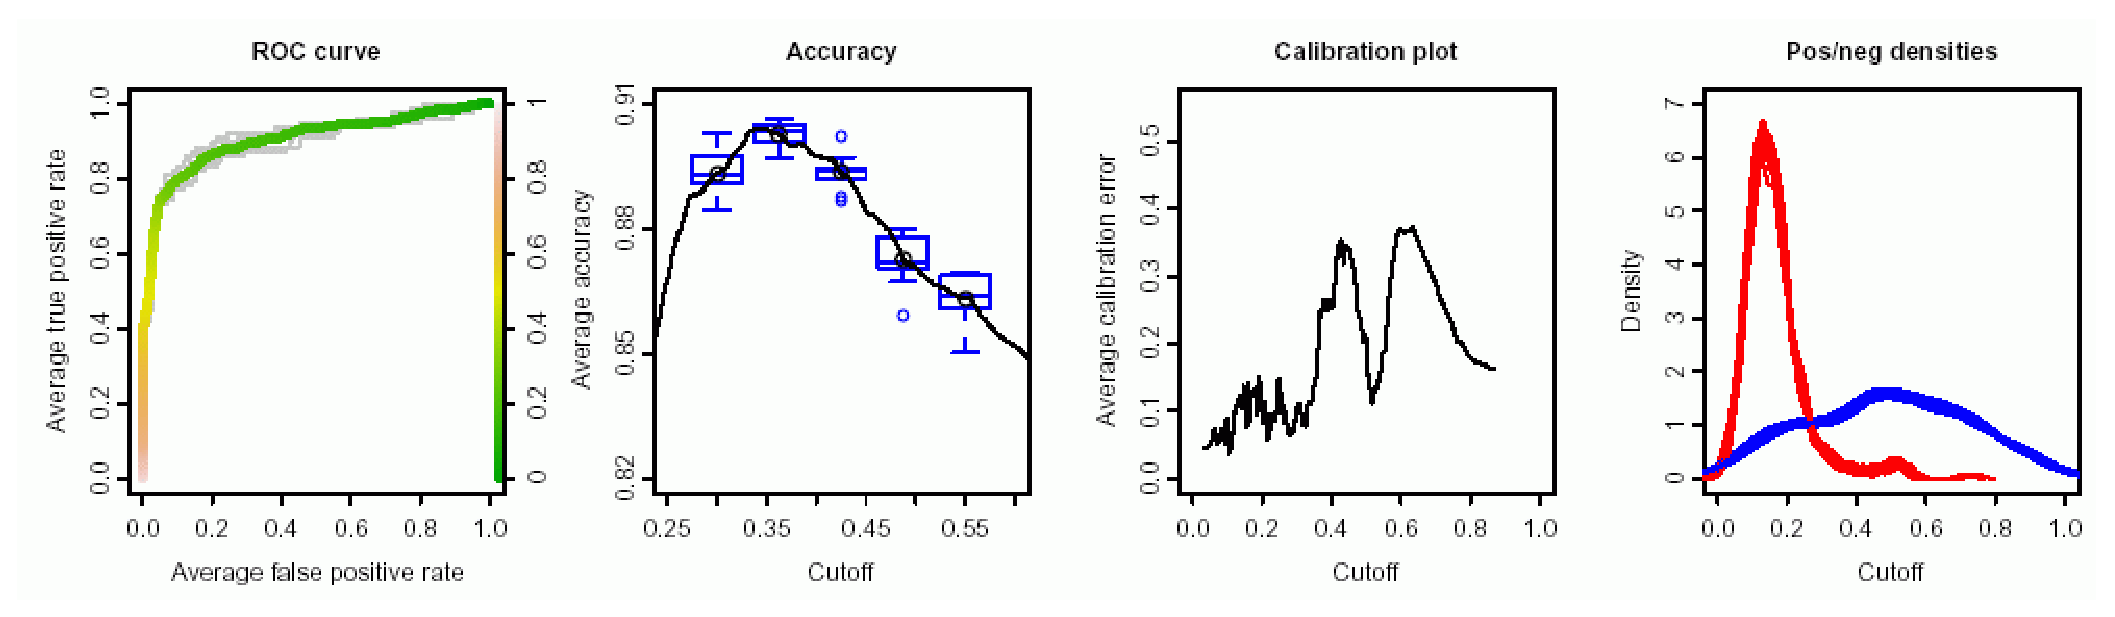
\includegraphics[height=5cm]{./images/ROCR_samples.eps}}
  \caption{Samples of ROC curves}\label{fig:ROCR_1}
\end{figure}

\section{Packages for data analysis}
\label{sec:pack-data-analys}

\subsection{BSDA}
\label{sec:bsda}
Basic Statistic and Data Analysis\footnote{\url{
http://cran.r-project.org/web/packages/BSDA/index.html}}
This contains the data and some statistic functions from the book 'Basic
statistics and data analysis', Kitchens, L. J. (2003) , Duxbury.

\subsection{coin}
\label{sec:coin}

coin stands for COnditional INference procedures in a permutation test
framework\footnote{\url{http://cran.r-project.org/web/packages/coin/index.html}}.
This package contains Conditional Inference Procedures for the general
independence problem including two-samples, K-sample (non-parametric
ANOVA), correlation, censored, ordered, and multivariate problems


\subsection{DAAG}
\label{sec:daag}

DAAG stands for Data Analysis And Graphics data and functions which
includes all functions described in the book Maindonald, J.H. and
Braun, W.J. (2003, 2007) "Data Analysis and Graphics Using R".

\subsection{nortest}
\label{sec:nortest}

nortest is being used to test for
normality\footnote{\url{http://cran.r-project.org/web/packages/nortest/index.html}}

\begin{lstlisting}
pearson.test(x, n.classes = ceiling(2 * (n^(2/5))), adjust = TRUE)
\end{lstlisting}

\subsection{sciplot}
\label{sec:sciplot}

The package "sciplot" is now available for download from CRAN. This
package includes a collection of functions that create graphs with
error bars for data collected from one-way or higher factorial
designs, as well as a function to plot bifurcation diagrams resulting
from analysis with XPPAUTO. The functions in this package replicate
some of the functionality of {\bf plotmeans()} from the package {\it gplots}, with
differences in the treatment of two-way and higher designs. Example
graphs can be seen at: \url{http://mutualism.williams.edu/sciplot}

\begin{figure}[htb]
    \centerline{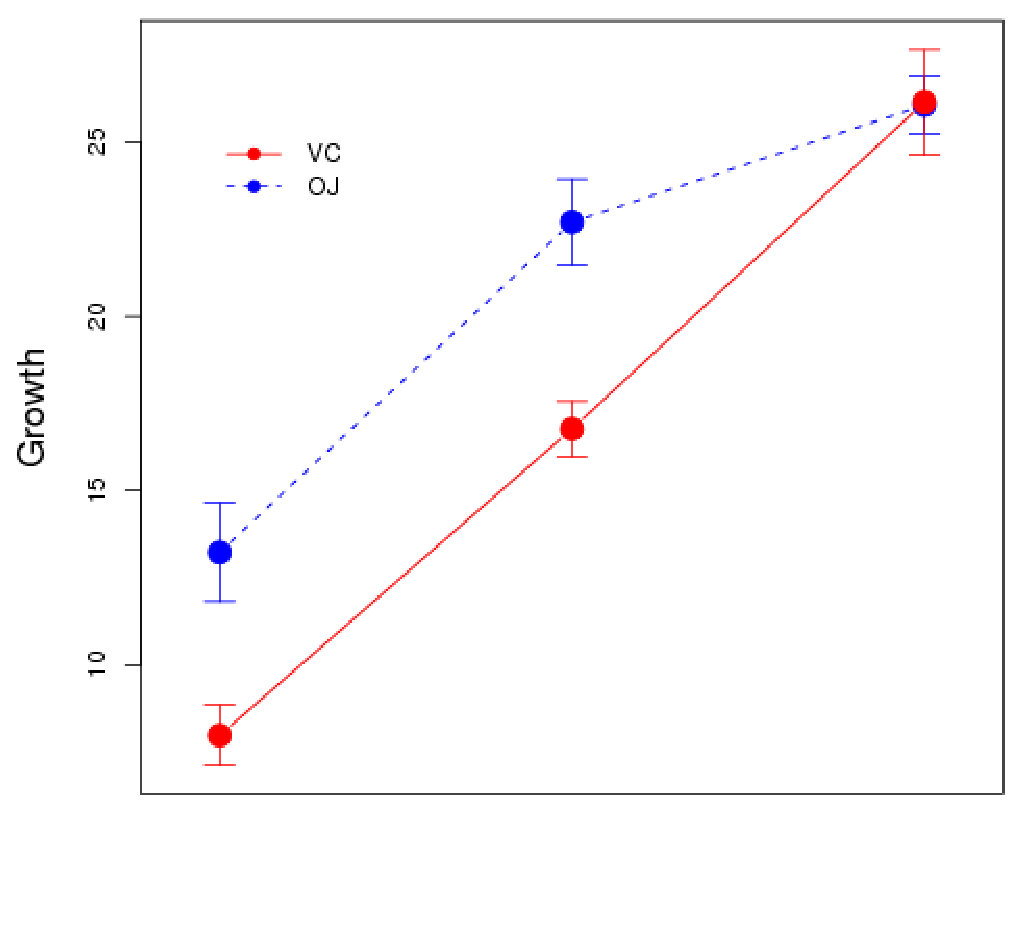
\includegraphics[height=5cm]{./images/sciplot_samples.eps}}
    \caption{Samples from sciplot}\label{fig:sciplot_1}
  \end{figure}

\section{Packages with problem solving}
\label{sec:pack-with-probl}

\subsection{plyr}
\label{sec:plyr}

{\bf plyr} is a set of tools that solves a common set of problems: you
need to break a big problem down into manageable pieces, operate on
each pieces and then put all the pieces back together.  It's already
possible to do this with {\bf split()} and the {\bf apply()}
functions, but plyr just makes it all a bit easier with:

\begin{itemize}
\item consistent names, arguments and outputs

\item input from and output to data.frames, matrices and lists

\item progress bars to keep track of long running operations

\item built-in error recovery

\item the choice of passing chunks as rows or as variables
\end{itemize}

plyr functions are named according to the type of object they input
(first letter) and output (second letter):

\begin{itemize}
\item   llply = from a list to a list
\item  alply = from an array (or vector, or matrix) to a list
\item  ldply = from a list to a data.frame
\item   \verb!d_ply! = from a data.frame, ignore output
\item and so on for llply, laply, ldply, \verb!l_ply!, alply, aaply,
  adply, \verb!a_ply!, dlply, daply, dply, \verb!d_ply!
\end{itemize}

plyr also provides:

\begin{itemize}
\item    m*ply which works in a similar way to mapply
\item   r*ply which works in a similar way to replicate
\end{itemize}

You can find out more at \url{http://had.co.nz/plyr/}, including a 20
page introductory guide\footnote{\url{http://had.co.nz/plyr/plyr-intro.pdf}}.


\section{Packages for model analysis}
\label{sec:pack-model-analys}

\subsection{Caret}
\label{sec:caret}

caret is a package for {\it building} and {\it evaluating} a wide
variety of predictive models. There are functions for pre-processing,
tuning models using resampling, visualizing the results, calculating
performance and estimating variable importance. 

{\bf caretNWS} and {\bf caretLSF} are two parallel processing versions
that can reduce the training time when multiple compute nodes are
available.

The project is now hosted on
\href{http://caret.r-forge.r-project.org/}{R-Forge}.  The package
currently includes {\bf model tuning/resampling} for the following
models: lm, single trees (C4.5, rpart, ctree, logistic model trees),
mars (via earth), boosted models (ada, gbm, blackboost, glmboost,
gamboost, logitboost), bagged models (trees, earth, fda),
randomforests (randomforest and cforest), rule-based models (Ripper
and M5 prime), discriminant models (lda, fda, rda, ssda, slda), kernel
methods (lssvm, ksvm, rvm, gausspr), nnet, nnet with initial pca step,
multinom, pls, plsda, gpls, nearest shrunken centroids, the lasso, the
elastic net, supervised pca, knn, lvq and NaiveBayes.

Recent changes include:
\begin{enumerate}
\item Estimation of class probabilities from PLS discriminant analysis
  using Bayes rule (in addition to softmax)
\item Added predict.train and predit.list

\item More lattice plots to visualize resampling results (xyplot,
  stripplot, densitplot, histogram) 

\item User-specified performance metrics for resampling

\item User-specified algorithms for determining the optimal tuning
  parameters (instead of highest/lowest)

\item A CHANGES files now exists to track the specifics of the version
  changes 
\end{enumerate}

\section{Packages for machine learning}
\label{sec:pack-mach-learn}

\subsection{e1071}
\label{sec:e1071}

Functions for latent class analysis, short time Fourier transform,
fuzzy clustering, support vector machines, shortest path computation,
bagged clustering, naive Bayes classifier, ...  
 
\subsection{GALGO}
\label{sec:galgo}

A package for multivariate variable selection using Genetic Algorithm
\url{http://www.bip.bham.ac.uk/bioinf/galgo.html }

\subsection{LearnBayes}
\label{sec:learnbayes}

\url{http://bm2.genes.nig.ac.jp/RGM2/pkg.php?p=LearnBayes}

\section{Packages in epidemiology}
\label{sec:pack-epid}

\subsection{epitools}
\label{sec:epitools}

\url{http://cran.r-project.org/web/packages/epitools/index.html}

\section{Packages in psychology}
\label{sec:packages-psychology}

\subsection{psych}
\label{sec:psych}


A number of routines for personality, psychometrics and experimental
psychology
research\footnote{\url{http://cran.r-project.org/web/packages/psych/index.html }}.
Functions are primarily for scale construction using factor analysis,
cluster analysis and reliability analysis, although others provide
basic descriptive statistics

\begin{lstlisting}
> install.packages("psych")
> library(psych)
\end{lstlisting}

Some useful functions:
\begin{lstlisting}
geometric.mean()
harmonic.mean()
\end{lstlisting}



%%% Local Variables: 
%%% mode: latex
%%% TeX-master: "R_language"
%%% End: 

\section{Miscellaneous}
\label{sec:miscellaneous}

\subsection{survey}
\label{sec:survey}

\url{http://faculty.washington.edu/tlumley/survey/}

\subsection{a}


\url{http://www.braju.com/R/}

\subsection{gplots}
\label{sec:gplots}


\section{Packages for bioinformatics}
\label{sec:pack-bioinf}

\subsection{Bioconductor}
\label{sec:bioconductor}

Bioconductor project (www.bioconductor.org)
